Utilizing a panel DID identification strategy, I first measure the impact of the TOU prices on 30-minute-interval household electricity consumption. To obtain the Average Treatment Effect (ATE) for each half-hour interval, I estimate the following specification:
\begin{equation}
\begin{split}
    \textit{kWh}_{itw} \ 
    & = \ \beta_{w} \mathbb{1}\big[ \text{Treatment \& Post} \big]_{it} \ + \ \alpha_{iw} \ + \ \gamma_{tw} \ + \ \delta_{m} \ + \ \epsilon_{itw}
\end{split}
\label{Eq:Model-Specification_Half-Hourly-Average-Treatment-Effects}
\end{equation}
The term $kWh_{itw}$ is the electricity consumption by household $i$ on the day $t$ during the half-hourly time window $w$. The indicator variable $\mathbb{1}\big[ \text{Treatment \& Post} \big]_{it}$ is equal to 1 only if household $i$ is in the treatment group and the day $t$ is in the treatment period. The terms $\alpha_{iw}$, $\gamma_{tw}$, and $\delta_{m}$ are household-by-half-hourly-interval, day-of-sample-by-half-hourly-time-window, and month-of-year fixed effects, respectively. In the specification, the point estimates of $\beta_{w}$, representing the ATE for each 30-minute interval $w$, are the parameters of interest. I cluster the standard errors at the household and the day of experiment levels to correct for serial correlation.

\afterpage{
    \begin{figure}
        \centering
        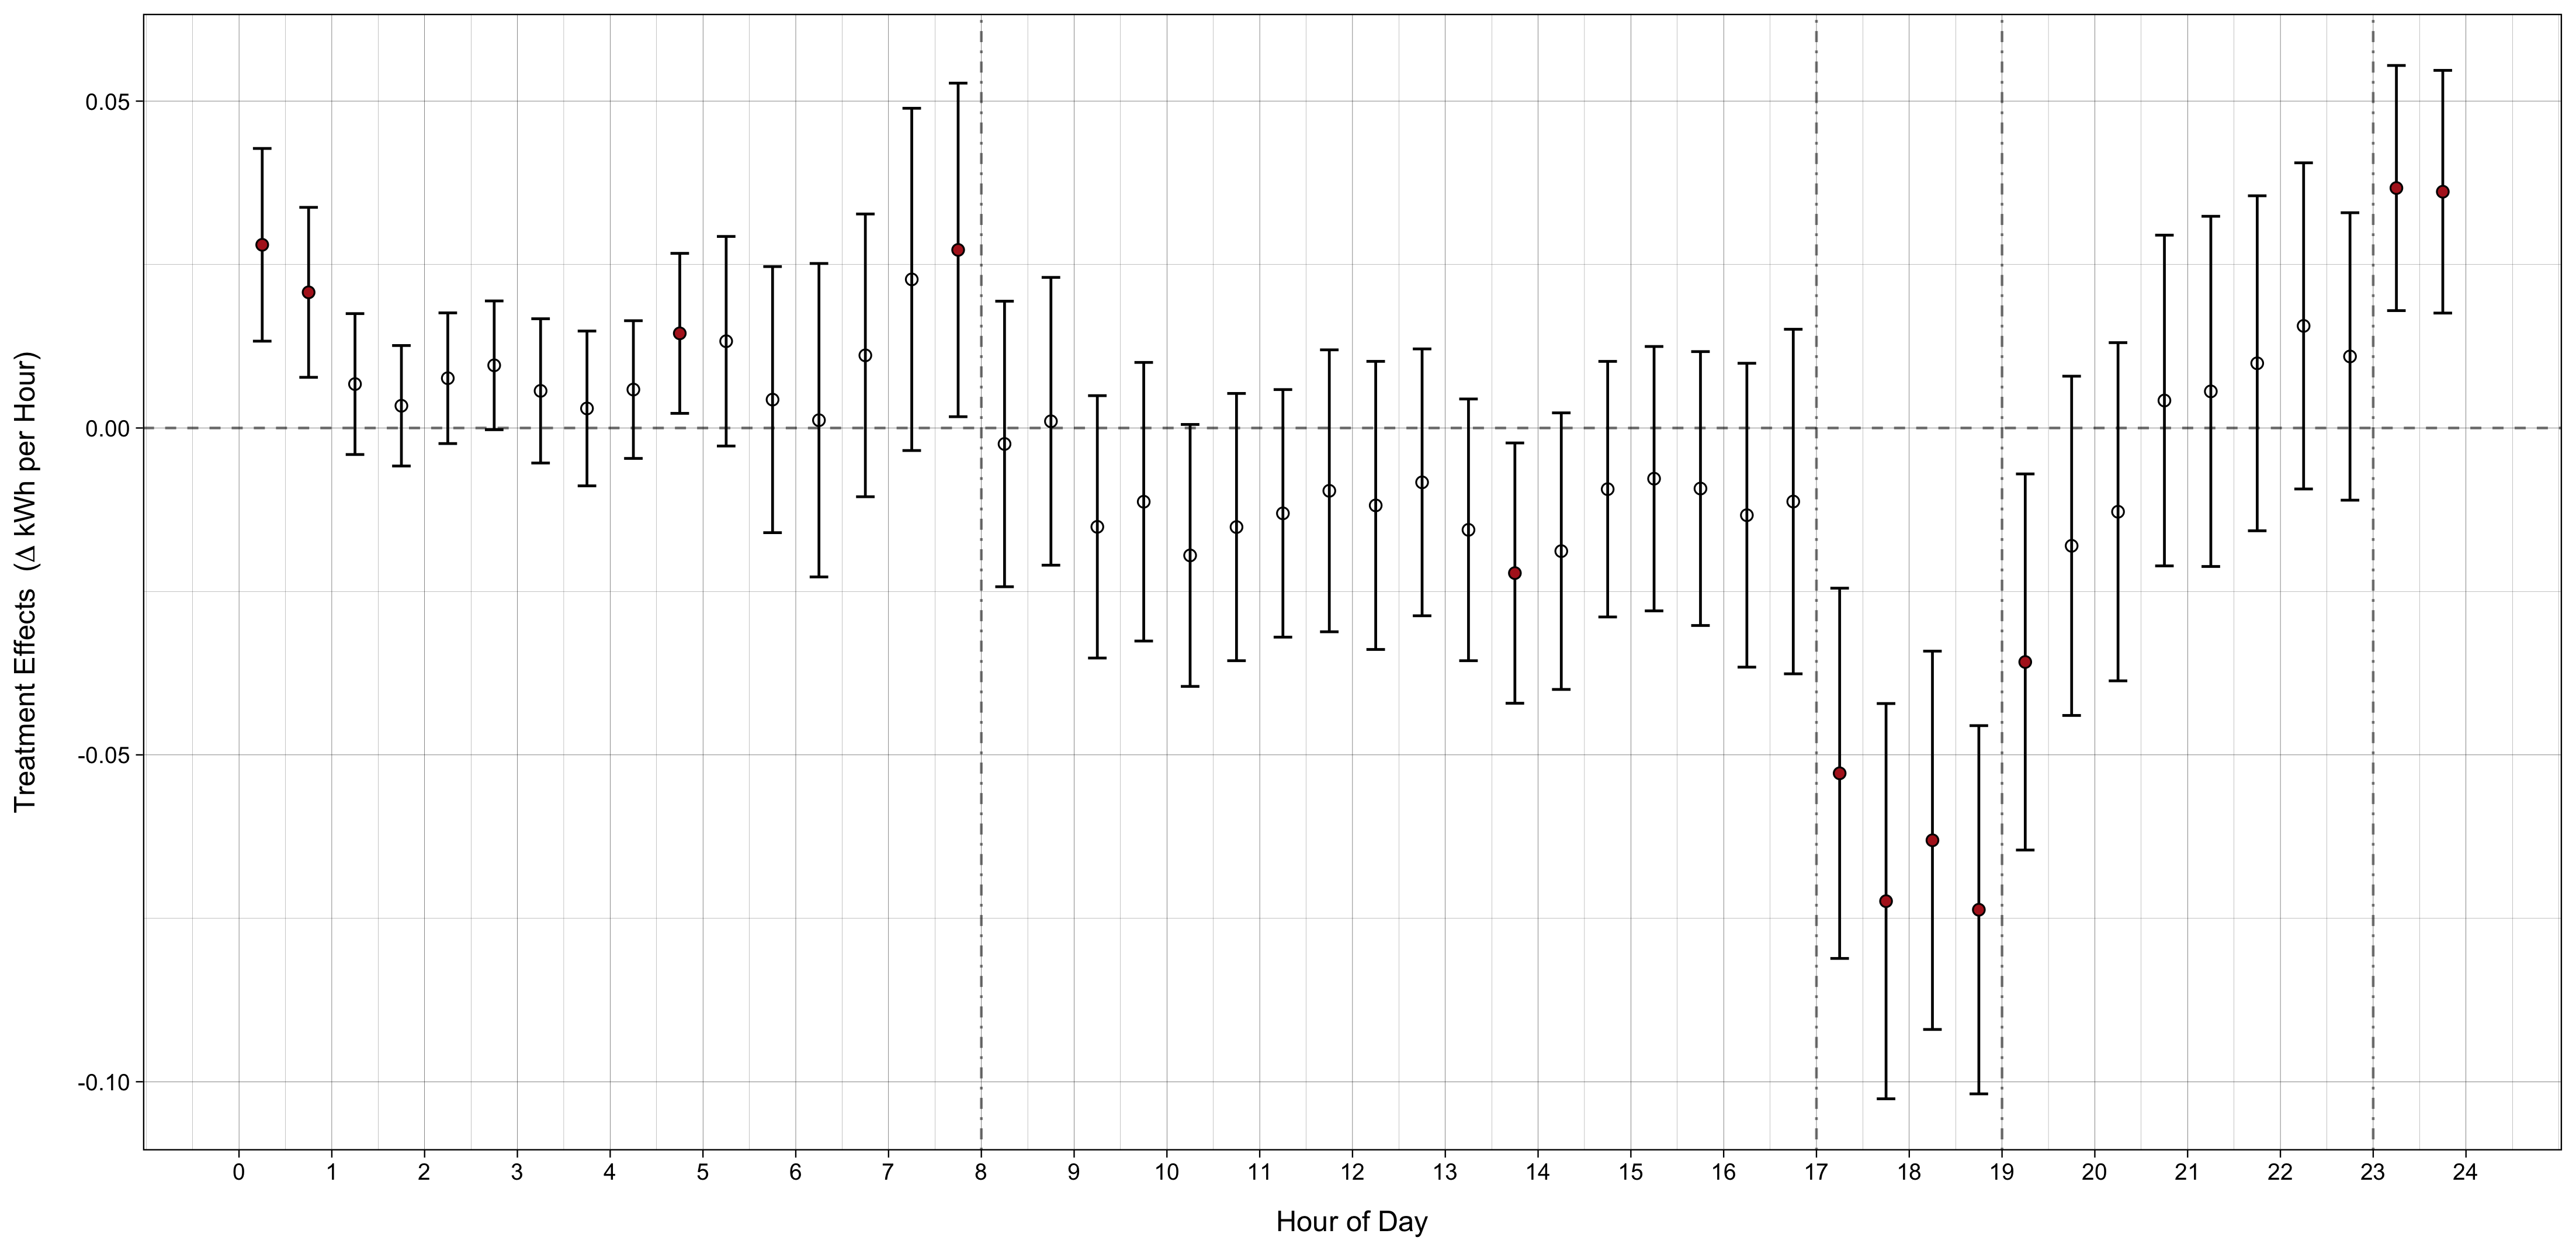
\includegraphics[scale = 0.10]{03_Chapter-2/00A_Figures/Figure_Time-Profile-of-Half-Hourly-ATEs.png}
        \caption{Half-hourly Average Treatment Effects}
        \caption*{
            {\small
            \textit{Note}: This figure depicts the time profile of half-hourly average treatment effects with 95\% confidence intervals. Standard errors are clustered at the household and date levels to adjust for serial correlation. As clearly illustrated, the treated households significantly reduced their electricity consumption during peak hours. A more interesting phenomenon is that they reduced their electricity consumption in hours leading up to and following the peak rate period, during which the applicable unit rate was lower than the flat rate in the baseline period, even though most of the estimated treatment effects are statistically insignificant in those hours. 
        }}
        \label{Figure:Half-Hourly-Average-Treatment-Effects}
    \end{figure}
}
Figure \ref{Figure:Half-Hourly-Average-Treatment-Effects} summarizes the estimated ATEs in the form of a time profile. As already demonstrated in \cite{Peaking-Interest:How-Awareness-Drives-the-Effectiveness-of-Time-of-Use-Electricity-Pricing_Prest_2020}, peak hours (i.e., from 5:00 p.m. to 7:00 p.m.) show dominant electricity savings. The figure also demonstrates reductions in household electricity consumption not only in most of the meter readings prior to the peak rate period but also in three successive meter readings right after the period, even though the reductions, with two exceptions, are not statistically significant. The insignificant reductions in household electricity consumption are interesting because TOU prices in off-peak hours (i.e., prices in the night and day rate periods) were lower than the flat rate in the baseline period. The counterintuitive changes might indicate that households preemptively adjusted their consumption behavior to avoid the incident of paying higher prices. In other words, the peak-hour price increases under the TOU program were likely to cause some spillover effects in the hours leading up to and following the peak rate period. To explore whether households responded to the TOU program outside of the peak rate period as well or not, in the following empirical analysis, I will also pay attention to the off-peak hours, particularly the hours surrounding the peak rate period.
